\documentclass[a4paper,14pt]{article}

\usepackage[utf8]{inputenc}
\usepackage[spanish]{babel}
\usepackage[usenames]{color}
\usepackage{graphicx}
\usepackage{amsmath}
\usepackage[hidelinks]{hyperref}
\usepackage{multicol} 
\usepackage{appendix}

\begin{document}
\begin{center}
\begin{Huge}
Lista de cosas para hacer\\
Tipo portafolio 
\end{Huge}
\end{center}
[30/03/2020]

\begin{itemize}
\item Implementar programa\\
Hacer programa en python 3.6 mediante el programa PyCharm, utilizando el directorio
$$./Escrotorio/Tesis/Programas$$
\begin{enumerate}
\item Revisar los programas que tengo hasta ahora\\
Revise algunos programas de las carpetas ya menionada por este momento(30/03/2020) trabajare con el programa "\textit{modelo\_LLS\_02.py}" 

\item Modificar/crear un programa nuevo, y desglosar las tareas 
\end{enumerate}
\item Escribir documento (Tesis)
\begin{enumerate}
\item Revisar la información que tengo
\item Direccionar la finalidad del documento
\item Escribir
\item Presentarlo
\end{enumerate}
\item \textcolor{blue}{Cosas por hacer
\begin{enumerate}
\item Revisar el programa (Literatura e implementacion)
\item Analizar lo de la optimización (Programacion y literatura)
\end{enumerate}}
\end{itemize}
[31/03/2020]
\begin{itemize}
\item Programa\\
Revisado el programa del aritculo del 1994\footnote{A microscopic model of the stock market: cycles, booms, and crashes, Levy, Moshe and Levy, Haim and Solomon, Sorin, Economics Letters, 1994}, lo deje en la carpeta como modelo\_LLS\_02.py.\\
Problemas con la optimización de la función, solo use la función, de la libreria  \textit{scipy}, optimize.fmin(), al obtener la variable $x_op[i]$ luego se le agrega una variable aleatoria $\varepsilon$ y esta es la que define los dos modelos pues
\begin{enumerate}
\item $\varepsilon \rightarrow 0$ el modelo tiende a ser Homogeneo,y cuando
\item $\varepsilon \rightarrow 1$ el modelo se vuelve heterogeneo
\end{enumerate}
\end{itemize}
[31/03/2020]
\begin{itemize}
\item \textcolor{blue}{Hoy principalmente enfocado a optimizar ediante la libreria \textit{scipy}}\\
\quad Revisado un poco la información de la optimización, identificando que mi caso es un optimizacion seria
\begin{equation}
EU[w_h(i)] = \frac{1}{k}\sum^{k-n}_{j=1}\log{[(1-x)(1+r)w_h(i)+xw_{h}(i)(1+H(i,j))]}
\end{equation}
ó
\begin{equation}
EU[w_h(i)] = frac{1}{k}\sum^{k-n}_{j=1}\log{[w_h(i)(1+r)+xw_{h}(i)(H(i,j)-r)]}
\end{equation}
esto sujeto a $0.01\leq x \leq 0.99$\\
 Intentando utilizar 
\begin{itemize}
\item \textit{scipy.optimize.fminbound()} $\rightarrow$ Minimización limitada para funciones escalares
\item \textit{scipy.optimize.minimize\_ escalar()}
\end{itemize}
\textcolor{blue}{Ahora a implementar en el programa el algoritmo para optimizar}
\item \textcolor{red}{Revisar el material teorico, para saber donde estoy? y ademas comenzar a recopilar informacion para escribir el texto}
\item En la tarde intentar modificar el programa.\\ 
\textcolor{blue}{Implemente lo que encontre usando el comando \textit{scipy.optimize.fminboun()} y el programa si se obtiene la Figura (\ref{F1[30/03/2020]})}
\begin{figure}[h]
\centering
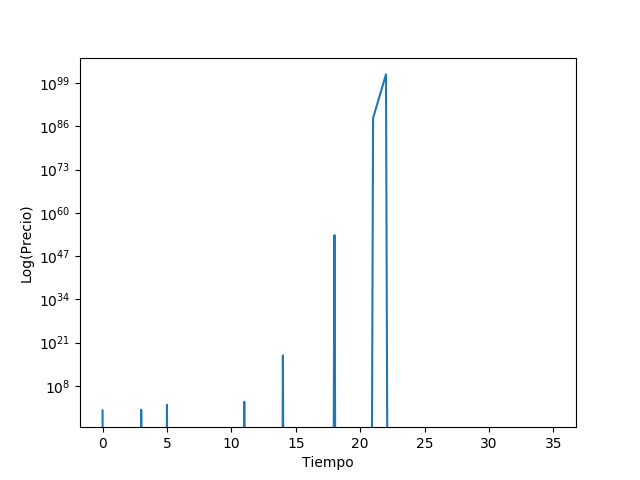
\includegraphics[scale=0.5]{Figure_1.png}
\label{F1[30/03/2020]}
\caption{Figura obtenida del programa con los siguientes valores $t=100$, $i=10$, $k=2$, $N_t=10000$}
\end{figure}

\item \textcolor{red}{Corregir el tema de las iteraciones, solo aparecen $\sim$ 25 siendo que lo itere 100}
\end{itemize}
[01/04/2020]
\begin{itemize}
\item Cmbiando el valor de interación, es decir bajando de $t = 100$  a $t= 30$ se obtiene la Fig.(\ref{F2[01/04/2020]})

\begin{figure}[h]
\centering
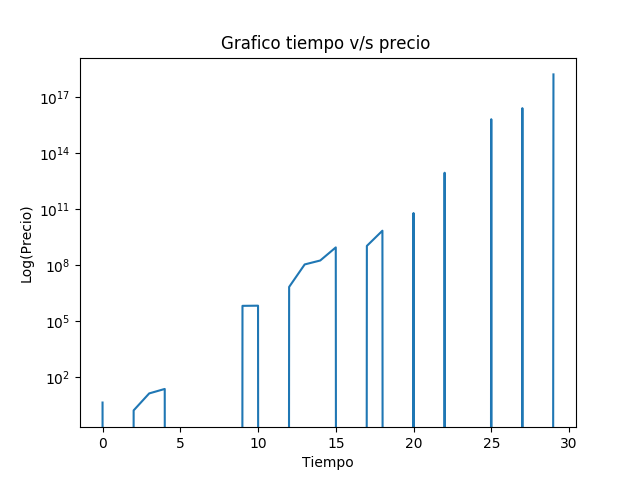
\includegraphics[scale=0.5]{Figure_2.png}
\caption{Figura obtenida del programa con los siguientes valores $t=30$, $i=10$, $k=2$, $N_t=10000$}
\label{F2[01/04/2020]}
\end{figure}
\item Todavía esta pendiente esta parte de la historia\\ 
Al revisar la información e intentado delimitar el topico ha tratar y así poder enfocarme efectivamente sobre el tema de '\textit{Toma de desición mediante redes neuronales y/o otro método}'\\
\begin{center}
\textit{Implementar un modelo con la misma dinámica que el modelo LLS, pero variar la forma de optimizar en primera instancia intentar utilizar:
\begin{enumerate}
\item Redes Neuronales
\item Alguna otro metodo nuevo para optimizar, ver si los grafos funcionan
\end{enumerate}}

\end{center}
\item \textcolor{red}{Revisar eldocumento teorico, elaborado para saber donde estoy? y ademas comenzar a recopilar informacion para escribir el texto}\\
\item \textcolor{red}{Además, hoy seguire mejorando el programa, en la tarde/noche, cosas a considerar para mejorar (por ahora)}
\begin{itemize}
\item \textcolor{blue}{generar leyenda en los graficos que contenga los parametros utilizados}\\
Agregue los comando y obtuve la grafica tipo (Fig. (\ref{F3[01/04/2020]})) que me muestra los valores de las variables empleadas
\begin{figure}[h]
\centering
%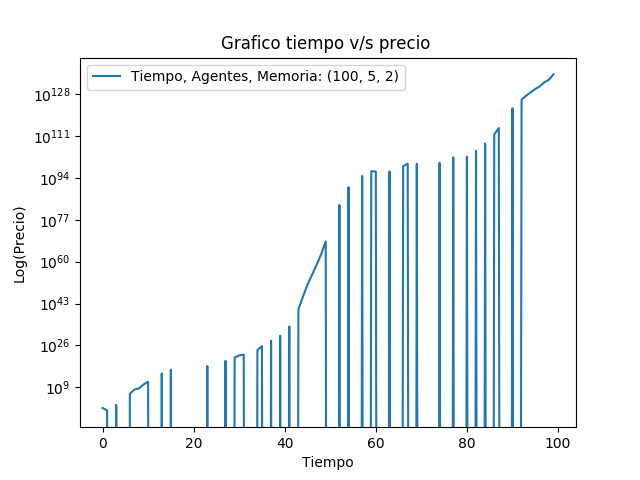
\includegraphics[scale=.5]{../../Graficas/Figura_3.png} 
\label{F3[01/04/2020]}
\caption{Figura con los datos de implementacion}
\end{figure}
\end{itemize}
\begin{itemize}
\item \textcolor{blue}{ aumentar la cantidad de iteraciones $t=(100, 200,\dots, 1000)$}\\
Con el programa actual, aumentará el valor con estos valores $t=100, 200, 300, 400, 500$ y el programa solo programa hasta $t\sim 100$. Además, le cambie la dirección para guardar las gráficas

\item \textcolor{red}{ Aumentar la cantidad de agentes en la iteración $i=(100,\dots, 500)$}
\item \textcolor{red}{ aumentar la capacidad de recordar $k$}
\item \textcolor{red}{ verificar la posibilidad de utilizar otra herramienta de optimización, otro metodo y comparar}
\end{itemize}
\end{itemize}
\newpage
[02/04/2020]\\
\begin{itemize}
\item \textcolor{blue}{Aumentar la cantidad de agentes en la iteración $i=(100,\dots, 500)$}\\
Logrado se generaron varios graficos con la misma forma solo que $t=100$ eso puede influir
\item \textcolor{blue}{Aumentar la capacidad de recordar $k=10,141,256$ (daatos utilizados en los articulos)}\\
se obtuvo los graficos(demoraron mucho)y el con k = 10 es normal ascendente, el con k= 141 da algo raro pues solo calcula unos datos y con k = 256 solo calcula t = 80
\textcolor{green}{Revisando el programa me confundi en la actulaizacion de los retornos}
\item \textcolor{blue}{intente agregar a la variable aleatoria del programa, un numero aletorio con una distribución normal, reemplazando por lo sgt; }
\begin{center}
x[i,t]=x\_op[i]+ np.random.normal($\mu$,$\sigma=0.24$)]\\
\quad Cambiar la optimizacion hay algo que no me da, al cambiar el valor de la definición de los numeros aleatorios, se coloca rara la cosa (graficas se cortan) 

\end{center}

\item \textcolor{red}{NECESARIO: Verificar la posibilidad de utilizar otra herramienta de optimización, otro metodo y comparar}
\item \textcolor{red}{Revisar el documento teorico, elaborado para saber donde estoy? y ademas comenzar a recopilar informacion para escribir el texto. Empezar a escribir el texto}\\
\end{itemize}
[04/04/2020]
\begin{itemize}

\item \textcolor{red}{NECESARIO: Verificar la posibilidad de utilizar otra herramienta de optimización, otro metodo y comparar}
\item \textcolor{red}{Revisar el documento teorico, elaborado para saber donde estoy? y ademas comenzar a recopilar informacion para escribir el texto. Empezar a escribir el texto}\\
\end{itemize}
[07/04/2020]
\begin{itemize}
\item Revisando el programa, cambie la definicion de la funcion a optimizar;
\begin{itemize}
\item Agregando un bucle con $k$  para que recorra todos los valores de H[i,j] 
\item Agregando la suma a la función suma y el parametro $k$ que divide 
\item Tengo un problema en la actualización de las historias
\end{itemize}
\item \textcolor{blue}{NECESARIO: Verificar la posibilidad de utilizar otra herramienta de optimización, otro metodo y comparar}
\begin{itemize}
\item Utilizar la libreria de CXopt de python que una libreria para realizar optimizacion convexa
y por lo que leí debo considerar que la optimización es; determinista, tiene una función objeto con restricciones (desigualdades) y descreta no lineal ($\log(w(i))$) 
\item Recordar que para encontrar un maximo/minimo, pues
$$
\frac{\partial}{\partial x}f=
\frac{\partial}{\partial x}[U(w(i))]=
\frac{\partial}{\partial x}\frac{1}{k}\sum^{k}\frac{\partial}{\partial} \frac{w(H-r)}{w(1+r)+x(H-r)}=0
$$
\begin{equation}
\frac{\partial}{\partial x} EU(w())=\frac{1}{k}\sum^{k}\frac{H-r}{(1+r)+x(H-r)}=0 \label{ec.raices}
\end{equation}
Seria interesante solo encontrar las raices de Ec.(\ref{ec.raices}) y tener de referencia las restricciones $0.01\leq x \leq 0.99$\\
\textcolor{red}{Implementar una de estas dos formas numericas}
\end{itemize}
\item \textcolor{red}{Revisar el documento teorico}, \textcolor{blue}{elaborado para saber donde estoy? y ademas comenzar a recopilar informacion para escribir el texto. Empezar a escribir el texto}\\
Encontre un trabajo en preceso que es del año 2020\\

M.Beikirch and T.Trimborn, \textit{'Novel Insights in the Levy-Levy-Solomon Agent-Based Economic Market Model'}, 2020.
El cuál se enfoca en utilizar un simulador e implementa el modelo LLS  
\end{itemize}

[08/04/2020]

\begin{itemize}
\item \textcolor{red}{Revisar el documento teorico, Hacer el cuerpo de la tesis;
\begin{enumerate}
\item Problema de investigación
\item Marco teórico
\item Metodología
\item Resultados
\end{enumerate}}
\item \textcolor{red}{Implementar una de estas dos formas numericas} (recordar Ec.(\ref{ec.raices}))
\item \textcolor{blue}{Corregi la actulización de retornos, agregando el termino de acciones en los dividendo }
\end{itemize}

[14/04/2020]

\begin{itemize}
\item \textcolor{blue}{Revisar el documento teorico. Hacer el cuerpo de la tesis;}
\begin{enumerate}
\item Problema de investigación
\begin{itemize}
\item De la pagina\footnote{http://www.une.edu.pe/Sesion01-Planteamiento\_del\_problema\_cuantitativo.pdf}\\
Reconemnado hacerlo en parrafos(c/ parrafo minimo diez lineas) debe existir secuencia lógica. Se emple el metodo deductivo e inductivo (de lo generico a lo especifico o en forma viceversa). Eneunciar el problema (presentar una descripción general de la situción objetivo de investigación) y formular el problema 
\item DE la pagina\footnote{https://becasyconvocatorias.org/planteamiento-problema-tesis/}
De manera general;
\begin{itemize}
\item Poner el problema en \textbf{contexto}(?` qué sabemos ya ?)
\item Describir la \textbf{cuestión precisa} que abordará la investigación (?` qué necesitamos saber?)
\item Mostrar la \textbf{revelancia} del problema (?`por qué necesitamos saberlo?)
\item Establecer los \textbf{objetivos} de la investigación (qupe haŕa para averiguarlo)
\end{itemize}

\begin{itemize}
\item Paso 1; Contextualizar el problema.\\
El enunciado del problema debe enmarcar su problema de investigación en su contexto particular y proporcionar algunos antecedentes sobre lo que ya se sabe al respecto.\\
Problemas de investigación teórica\\
Pensar en los antecedentes científicos, sociales, geográficos y / o históricos:\begin{itemize}
\item ?`Qué se sabe sobre el problema?
\item ?`El problema se limita a un cierto período de tiempo o área geográfica?
\item ?`Cómo se ha definido y debatido el problema en la literatura académica?
\end{itemize}
\item Paso 2; Muestra por qué es importante\\
?`por qué es importante que se resuelva el problema?. Esto no significa que tengas que hacer algo innovador o que cambie el mundo. Es más importante que el problema sea investigable, factible y aborde claramente un problema relevante en su campo.\\
Problemas de investigación teórica, para identificar por qué el problema es importante, pregunta:
\begin{itemize}
\item ?`Cómo la resolución del problema avanzará en la comprensión del tema?
\item ?`Qué beneficios tendrá para futuras investigaciones?
\item ?`El problema tiene consecuencias directas o indirectas para la sociedad?
\end{itemize}
\item Paso 3; Establecer tus fines y objetivos\\
Finalmente, el enunciado del problema debe enmarcar cómo pretende abordar el problema. Su objetivo no debe ser encontrar una solución concluyente, sino buscar las razones detrás del problema y proponer enfoques más efectivos para abordarlo o comprenderlo.\\ El objetivo es el propósito general de su investigación. Generalmente se escribe en forma infinitiva:
\begin{itemize}
\item El objetivo de este estudio es \textbf{determinar} …
\item Este proyecto tiene como objetivo \textbf{explorar} …
\item Mi objetivo es \textbf{investigar} …
    \end{itemize}
Los objetivos son los pasos concretos que tomará para lograr el objetivo:
\begin{itemize}
\item    Se utilizarán métodos cualitativos para \textbf{identificar} …
\item Usaré encuestas para \textbf{recopilar} …
\item Mediante el análisis estadístico, la investigación \textbf{medirá} … 
\end{itemize}  
\end{itemize}

\item De la pagina\footnote{https://www.scribbr.es/como-empezar-tfg/como-escribir-el-planteamiento-del-problema/}\\
Lo necesitas por dos razones principales:
\begin{itemize} \item El planteamiento del problema es el punto de partida de tu principal pregunta de investigación. \item El planteamiento del problema te da enfoque y te obliga a centrarte en algo muy concreto.
\end{itemize}
\begin{enumerate}
\item  Identifica una problemática general en el campo de tu tesis\\
Empieza por identificar un problema en el que te gustaría centrarte.
\item Infórmate acerca del problema\\
Desarrollar la compresión necesaria para identificar el aspecto del problema que tratará\\
Dependiendo del tema, tu investigación puede incluir: consultar la literatura y otras fuentes de información relevantes o hablar con expertos. Al realizar esta investigación, ten en cuenta las siguientes preguntas:
\begin{itemize}
\item  Contexto: ?`Quién tiene un problema y cuándo/dónde surge? ?`Cuál es la causa del problema (por ejemplo, proviene de una investigación anterior o se relaciona con un cambio en algún factor)?
\item  Antecedentes: ?`Qué se sabe sobre el problema? ?`Qué tienen que decir los investigadores y otros individuos involucrados? ?`Qué se ha hecho para resolver el problema? ?`Alguna solución ha tenido éxito? De ser así, ?`por qué? ?`Se ha enfocado en alguna causa en particular?
\item Especificidad: ?`Qué es exactamente lo que vas a ayudar a resolver? ?`Qué no abordarás?
\item Relevancia: ?`Por qué es importante para la sociedad o la profesión resolver tal problema? ?`Qué pasará si no se resuelve? ?`Quién sentirá las consecuencias?
\end{itemize}
\item Una vez que hayas avanzado un poco en la investigación y hayas respondido a las preguntas anteriores, deberías tener una idea más concreta de lo que, dentro del problema más vasto, te gustaría abordar. El siguiente paso es transformar esto en el planteamiento del problema que quieres ayudar a resolver y, así, demostrar la relevancia de tu investigación.

El planteamiento del problema no tiene que limitarse a una sola oración. También puede describirse en un breve párrafo.
\end{enumerate}
\end{itemize}
\end{enumerate}
\end{itemize}
[15/04/2020]
\begin{itemize}
\item \textcolor{blue}{Revisar el documento teorico. Hacer el cuerpo de la tesis;}
\begin{enumerate}
\item Problema de investigación
\item Marco teórico
\end{enumerate}
\end{itemize}
[27/4/2020]
\begin{itemize}
\item \textcolor{blue}{Investigar como hacer las partes del documento teorico, el cuerpo de la tesis;}
\begin{enumerate}
\item Problema de investigación
\item Marco teórico
\begin{enumerate}
\item sacada de \footnote{https://www.uv.mx/veracruz/insting/files/2013/02/propuesta-de-tesis-final.pdf}\\
En este apartado se deberá analizar todo aquello que se ha escrito acerca del objeto de estudio: ?`qué se sabe del tema? ?`qué estudios se han hecho en relación a él? ?`desde qué perspectivas se ha abordado?.\\
Deberia contemplar los siguientes aspectos:
\begin{enumerate}
\item Delimitar el área de investigación;
\item Sugerir guías, áreas, nichos o líneas de investigación;
\item Hacer un compendio de conocimientos existentes en el área que se va a investigar;
\item Expresar proposiciones teóricas generales, postulados, marcos de referencia;
\item Ayudar a prevenir errores que se han cometido en otros estudios;
\item Orientar sobre cómo habrá de llevarse a cabo el estudio;
\item Ampliar el horizonte del estudio y guiar al alumno para que éste se centre en su problema evitando así posibles desviaciones del planteamiento original; \item Proveer un marco de referencia para interpretar los resultados del estudio.
\end{enumerate}
Las  etapas pertinentes serian,  la  revisión  crítica de la literatura correspondiente, pertinente y actualizada, y posteriormente, la adopción de una teoría o desarrollo de una perspectiva teórica
\item De la pagina de recursos digitales de la PUC\footnote{http://informedecaso.educacion.uc.cl/estructura-a/estructura-a-introduccion}\\
presentan los principales elementos de la teoría que luego utilizarás para analizar e interpretar la evidencia. En un marco teórico, los diversos aspectos de las teorías, tales como definiciones y características, deben aparecer explicados y discutidos, recurriendo a citas desde las fuentes.\\Estrategias para planificar el marco teorico. Par simplificar la redaccion del marco teorico, es imprescindible planificar. Se sugioere
\begin{itemize}
\item Haz una lista de los temas que vas a abordar, referentes teoricos más adecuados par el caso de estudio. Escoger un orden para presentarlos de gorma lógica. General a lo particular, agrupacion por tematicas similares, ordenacion cronologica
\item Colocar subtitulos por si es muy extensa la informacion
\item Ten presente los titulos y subtitulos de los textos, en funcion a temas y su ordenacion logica
\item Se basa en fuentes academicas, medintes citas o parafrasis (propia palabras los que dicen en los textos). Definir previamente y tenerlas en la manos cuando se escribe
\item Acá se debe constrastar y evaluaar las diferentes teorias y conceptos que serviran pra el analisis de la evidencia. Importante preguntarse ?`Qué elementos en común y qué diferencias existen entre estas aproximaciones? ?`Cuáles de estas teorías me parecen más productivas (útiles) para interpretar mis datos? ?`Por qué?
\item Cuando comiences a escribir, ten la flexibilidad de adaptar o modificar tu planificación
\end{itemize}
\item Elementos de metadiscurso que te pueden ayudar a escribir tu marco teorico
\begin{itemize}
\item EXPRESIONES PARA SECUENCIAR E INTRODUCIR TEMAS\\
Primero - en primer lugar - por último - los siguientes - segundo - a continuación - para continuar - en seguida - entonces - tercero - para comenzar - finalmente - por último - otro - también - además\\
    En cuanto a (...) - Con respecto a (...) - Respecto de (...)
\item EXPRESIONES PARA INTRODUCIR ELEMENTOS TEORICOS DESDE LOS TEXTOS\\
Señala - plantea - manifiesta - considera - señala - argumenta - propone - sugiere - muestra - explica - demuestra - describe - expone - reporta - discute - desarrolla - estudia - critica - contraargumenta - niega - piensa (si se expone un punto de vista) - encuentra (si se expone un hallazgo).\\
Para el autor - desde esta perspectiva - según x - a partir de este modelo/teoría planteamiento - en respuesta a - en oposición a

\item EXPRESIONES A EVITAR\\
    Evita utilizar verbos de reporte orales, tales como “dice” o “menciona”. Son poco precisos, ya que estás citando ideas desde fuentes escritas.\\
    También evita el neologismo “evidenciar”. Si quieres decir que gracias al texto algo se hizo evidente o se puso de manifiesto, prefiere las expresiones “relevar” o “poner en evidencia”.
\end{itemize}
\end{enumerate}
\item Metodologia
%\begin{enumerate}
%\item De acá \footnote{https://www.uv.mx/veracruz/insting/files/2013/02/propuesta-de-tesis-final.pdf}\\
La metodología aclara –en forma muy detallada– los pasos y procedimientos utilizados para  llevar  a  cabo  la  investigación.  Así  mismo,  debe  incluir  paso  a  paso  la  explicación  de  todos  los  aspectos  necesarios  para  reproducir  o  repetir  la  investigación,  aquí  debe  quedar  muy claro el ‘cómo’ de la investigación.\\
Al escribir la tesis o al publicar los resultados de la investigación, la metodología debe escribirse en pasado explicando cómo se llevó a cabo la investigación.\\
La  metodología  cumple  varias  funciones,    primero  debe  esbozar  la  forma  en  que  se  desarrolló todo el proceso, con el mayor número de detalles posibles, indicandoel personal que  colaboró,  así  como  el  material  y  equipo    que  se  empleó  para  el  desarrollo  del  proyecto  de investigación.
\item sacado de la ayuda de PUC\footnote{http://informedecaso.educacion.uc.cl/estructura-a/estructura-a-metodologia}\\
Se explicita de qué modo obtuviste tus datos y cómo realizaste los análisis.
\begin{itemize}
\item La metodología se escribe en pasado. Se entiende que estás reportando un proceso de investigación que ya hiciste.
\item Aunque te pidan escribir la metodología primero, cuando ya hayas terminado el trabajo vuelve a revisarla y asegúrate que efectivamente describa los procesos hechos.
\item Existen diferentes modos de organización para esta sección del texto. Algunos lo harán por fases (ej: Fase 1: Recogida de datos) y otros por tema (ej: Muestra, Instrumentos, Procedimientos de análisis, etc.). Cualquiera sea el estilo que prefieras, asegúrate de ser consistente en la redacción.
\item Es obligatorio reportar:\\- Cuál es la muestra\\- Cómo la escogieron o delimitaron\\- Qué instrumentos y procedimientos utilizarán para observar y caracterizar. Si debes aplicar tests o pruebas, debes indicar el nombre y el autor del instrumento. Si van a construirlos ustedes, deben indicar cómo se elaboraron y añadirlos en un anexo al final del informe.
\end{itemize}
%\end{enumerate}
\item Resultados\\
%El análisis de un informe de caso examina detalladamente los componentes de un problema u objeto de estudio identificado en la realidad, estableciendo relaciones entre las evidencias recogidas y los fundamentos teóricos más adecuados. En general, el análisis es la sección a la que los profesores atribuyen mayor importancia en un informe de caso, ya que en esta se comprueba si los alumnos son capaces de “leer la realidad” desde el punto de vista de las teorías estudiadas durante el curso.
\begin{itemize}
%\item Estrategias para planificar el analisis\\
%Al momento de escribir tu análisis, es útil que te hagas algunas preguntas fundamentales que te ayudarán a planificar y ordenar tus ideas:
%
%¿Qué evidencias he recabado?
%¿Cuáles de estos datos me parecen más interesantes?
%¿Cuáles son las teorías estudiadas en el curso que me sirven para explicar estas evidencias? ¿Necesito buscar otras?
%Al escribir tu marco teórico dividiste tu texto en distintas secciones temáticas, asignaste títulos para describir el tema de cada sección, y las organizaste lógicamente. Si tu marco teórico está bien construido, este te permitirá dar cuenta de los distintos elementos o dimensiones del caso que estás estudiando. Así, aunque el análisis emerge de los hallazgos más interesantes que aparecen en tus datos, resulta coherente seguir el mismo orden lógico y temático que has determinado en tu marco teórico.
%\begin{center}
%RECORDATORIO\\
%Es posible que al revisar tus datos descubras que tu marco teórico no te permite dar cuenta de todos los elementos de la realidad que estás observando. En ese caso, te recomendamos revisar tu marco para integrar los elementos teóricos que hacen falta y, tal vez, modificar el orden en que lo has organizado.
%\end{center}
%Para asegurarte de lograr, en todo momento, establecer relaciones entre tus evidencias y la teoría, puedes recordar los siguientes pasos:
%\begin{enumerate}
%\item Enunciar el tema o aspecto relevante.Introduce el tema que vas a analizar por medio de una oración tópica, por ejemplo, “En cuanto al desarrollo...”, “Las tareas escritas por los niños muestran…”, etc. Cuando hagas referencia a la evidencia que has recabado, debes señalar claramente dónde está ese material. Usa los términos técnicos discutidos en el marco teórico.
%\item Citar la evidencia e incorporar un fragmento.
%Es mejor incluir directamente un fragmento de la evidencia que muestre lo que estás explicando, antes que simplemente remitir a los anexos. Haz click aquí para saber más sobre cómo integrar la evidencia.
%\item Interpretar la evidencia desde la teoría.
%Un análisis debe ir más allá de la mera identificación de fenómenos. Debes intentar proponer una interpretación interesante de las causas o implicancias del fenómeno observado. Utiliza los conceptos técnicos que introdujiste en el marco teórico y haz referencia a los autores.
%
%\item En algunos casos, conviene, al final del análisis, hacer una integración de los diversos elementos observados, a modo de cierre.
%En algunos casos, conviene hacer una integración de los diversos fenómenos analizados, a modo de cierre.
%\end{enumerate}
\item Elementos de metadiscurso que te ayudaran a escribir\\
EXPRESIONES PARA ORGANIZAR SECCIONES DEL ANÁLISIS
\\En primer lugar- En segundo lugar - De acuerdo a - Las evidencias recogidas - los principales hallazgos - Por otra parte - En relación a [dimensión estudiada] - En lo que respecta a...\\
EXPRESIONES PARA INTRODUCIR EJEMPLOS\\
como se observa en el siguiente ejemplo - este fragmento de [ej.: entrevista] pone en evidencia - lo anterior sugiere - el siguiente ejemplo muestra - esto se puede observar en - el fragmento anterior sugiere - esto se ilustra claramente en el ejemplo siguiente\\
EXPRESIONES PARA COMENTAR O INTERPRETAR A PARTIR DE REFERENTES TEÓRICOS\\
    de acuerdo con la teoría de - desde el punto de vista de [autor o teoría] esto sugiere que - tal como propone [autor o teoría], esto puede ser interpretado - [autor o teoría] explica que
\item \textcolor{blue}{En esta parte del texto utiizare las herramientas encontradas en la pag\footnote{http://informedecaso.educacion.uc.cl/estructura-a/estructura-a-introduccion}} 
\end{itemize}
\end{enumerate}
\item \textcolor{blue}{Realizar breve busqueda bibliografica sobre articulos que hablen del tema}\\
Impresos los ordenes cronologicamente, tengo varios 13 articulo/libros/documentos que tratan el tema o mehor dicho, en su referencia mencionan el primer artículo ('\textit{\textbf{A microscopic model of the stock market: Cycles, booms and crashes}}'). Por ahora, revisaré el conputador y la memoria externa para saber que articulos tengo y tomare de referencia el primer artículo publicado del tema y buscaré algunas referencias más.
\item \textcolor{red}{Programar, Terminar primera version del programa, y hacer variaciones}
\end{itemize}
[28/04/2020]
\begin{itemize}
\item Realizar breve busqueda bibliografica sobre articulos que hablen del tema. De acuerdo con este punto, ordené los aritculos que tenia impresos, en la carpeta el PC y en la memoria externo con la que cuento encontrando una cantidad de 34 articulos, libros y tesis que trata/mencionan el tema del model Levy-Levy-Solomon. \\
\textcolor{blue}{Pertinente hacer una lista digital de los artículos y enfocar el trabajao de leer los que no he leido y vincularlos para escribir el \textit{Cuerpo de la Tesis}}
Mas optimo, sacar foto a la lista que hice en papel, estan en esta misma carpeta son tres documentos (1\_l.png, 2\_l.png, 3\_l.png)
\item \textcolor{red}{Programar, Terminar primera version del programa, y hacer variaciones}
\end{itemize}
[30/04/2020]
\begin{itemize}
\item \textcolor{blue}{Realizar una revisión y separar en aarticulos que mencionan el modelo y los que incorporan nuevos datos }. Realice la revicion general, para saber si todos los aritculos que tenia en el computador hablaban del modelo o solo lo mencionaba y encontre que tengo en realidad $35$ articulos que mencionan el tema de los cuales 
\begin{itemize}
\item 3 solo mencionan el modelo LLS
\item 4 que mencionan el modelo pero el contexto es ma de revision de avances en el aerea
\item 8 articulos que trabajan inscpirado en el modelo LLS
\item 15 articulos que entregan informacion nueva sobre el modelo LLS(*)
\end{itemize}
\item \textcolor{red}{hacer resumen y escribir}
\item \textcolor{red}{Programar, Terminar primera version del programa, y hacer variaciones}
\item Arregle algunos comandos de latex, lo que consegui fue separar el archivo principal en varios documentos separados, que me ayudaran a trabajar puntualmente cada capitulo. Además, copie toda la bibliografia que debo leer ahora esos documentos que hablan del modelo basic(*)
\end{itemize}
[03/05/2020]
\begin{itemize}
\item \textcolor{blue}{Hacer resumen y escribir}, resumen en el cuaderno naranjo
\begin{itemize}
\item Listo leído, \textit{A microscopic model of the stock market}
\item Listo leído, \textit{Microscopic simulation of the stock market: the effect of microscopic diversity}
\item Listo leído \textit{The complex dynamics of a}
\end{itemize}
\item \textcolor{red}{Escribir, cuerpo de la tesis }
\item \textcolor{red}{Programar, Terminar primera version del programa, y hacer variaciones}
\end{itemize}
[13/05/2020]
\begin{itemize}\item \textcolor{red}{Escribir, cuerpo de la tesis }
\item \textcolor{red}{Terminar de leer los articulos}
\item \textcolor{red}{Programar, Terminar primera version del programa, y hacer variaciones}
\end{itemize}
[29/05/2020]
\begin{itemize}
\item \textcolor{red}{Programar principalmente; terminar el programa}
\end{itemize}
\end{document}
